\documentclass[11pt,
xcolor={svgnames},
hyperref={colorlinks,citecolor=green,linkcolor=DeepPink,anchorcolor=blue}
]{beamer}
\usetheme{Frankfurt}
%\usefonttheme{serif}
\usefonttheme[stillsansseriflarge,stillsansserifsmall]{serif}
%\usecolortheme{seahorse}
%\usecolortheme{rose}
%\setbeamerfont{title}{shape=\itshape,family=\rmfamily}
%\setbeamercolor{title}{fg=red!80!black,bg=red!20!white}

%\usepackage[super,square]{natbib}
\usepackage[utf8]{inputenc}
\usepackage[T1]{fontenc}
\usepackage{amsmath}
\usepackage{amsfonts}
\usepackage{amssymb}
\usepackage{graphicx}
\usepackage{xcolor}
\usepackage[linesnumbered,boxed,ruled,commentsnumbered]{algorithm2e}%%算法
\usepackage{listings}%%%%显示代码
\lstset{
	numbers=left,
	numberstyle=\tiny,
	keywordstyle=\color{blue!70},
	commentstyle=\color{red!50!green!50!blue!50},
	frame=single, 
	rulesepcolor=\color{red!20!green!20!blue!20},
	escapeinside=``
}
\usepackage{makecell}%改变表格横线样式, Xhline;Xcline


\DeclareGraphicsExtensions{.eps,.ps,.png,.jpg}%对于同名图片的优先顺序调用
\graphicspath{{graphics/}}%设置图片路径为当前路径下的graphics文件夹

\author{Liucheng Xu\\
	\smaller{2012080173}}
\title{Research on Content-Aware Collaborative Filtering}

\subtitle{Content-Aware Bayesian Personalized Ranking}

\logo{szulogo}

\institute{College of Computer Science and Software Engineering \\ Shenzhen University}

\date{\today}

\subject{Recommendation System}

\setbeamercovered{transparent}

\setbeamertemplate{navigation symbols}{}
\setbeamertemplate{footline}[frame number]{}

\begin{document}
	\maketitle
	
	\section*{Outline}
	\begin{frame}
		\tableofcontents[pausesections]
	\end{frame}
	
	
	\section*{Notations}
\begin{frame}
	\begin{table}[H]%[htbp]表格参数设置,固定位置
		\setlength\tabcolsep{2pt}
		\renewcommand\arraystretch{1.1}%改变行高
		\caption{Some notations}
		\label{tab1}
		\begin{center}
			
			\begin{tabular}{c|c}
				
				\Xhline{1.2pt}
				$s$                       &user number\\
				$t$                       &item number\\
				$k$                       &latent dimension (category number)\\
                $U,Y^u \in \mathbb{R}^{s\times k}$        &user latent matrix\\
				$V,Y^v \in \mathbb{R}^{t\times k} $       &item latent matrix \\
				$X \in \mathbb{R}^{t\times k}$            &ranking scores under categories\\
				$x_c \in X$                     &ranking score vector under category $c$\\
				$y^v_{*,c} \in Y^v$             & c-th column of $Y^v$\\
				$L\in \mathbb{R}^{t\times k}$   &ranking lists under categories\\
				$\rho \in \mathbb{R}^k$         & counters of category popularity\\
				$e \in \{u,v\}$                 & entity\\
				$A^e$                           &content feature of entities\\
				$W^e$                           &mapping matrix\\
				$Y^e$                           &entity latent matrix\\
				\Xhline{1.2pt}
				
			\end{tabular}
		\end{center}
	\end{table}
\end{frame}
	\section{引言}

\subsection{研究背景及意义}

互联网的出现和普及给用户带来了大量的信息, 满足了用户在信息时代对各种信息的需求, 但随着Internet的迅速发展而带来的网络上信息量的巨幅增长, 使得用户在面对大量信息时无法快速从中获得对自己真正有用的那部分信息。换言之, 在这种情况下人们对信息的使用效率反而降低了, 这就是所谓的信息过载(information overload)问题. 的确如此, 面对信息的汪洋大海, 人们往往感到无所适从, 信息过载已经成为一个不容忽视的问题.

目前, 应对信息过载的办法之一便是以搜索引擎为代表的信息检索系统, 比如国外的Google\footnote{\url{https://www.google.com/}}、国内的Baidu\footnote{\url{https://www.baidu.com/}}等, 它们在帮助用户从巨大的网络资源中获取信息方面发挥着极其重要的作用. 但对于使用搜索引擎的用户而言, 在使用同一个关键字搜索信息时, 在一段时间内所得到的结果都是相同的. 另一方面来看,信息及其传播是多样化的, 而用户对信息的需求是多元化和个性化的, 那么通过以搜索引擎为代表的信息检索系统获得的结果显然不能满足用户的个性化需求, 它们仍然无法很好地解决信息过载问题.

面对信息过载, 另外一个非常有潜力的办法是个性化的推荐系统, 它是根据用户的信息需求、兴趣等, 将用户所感兴趣的信息、产品、服务等推荐给用户的个性化信息推荐系统. 和搜索引擎相比, 推荐系统通过研究用户的历史行为与兴趣偏好, 进行个性化考量, 由系统发现用户的兴趣点, 从而引导用户发现自己的信息需求. 一个优秀的推荐系统不仅能为用户提供个性化的服务, 还能和用户之间建立密切关系, 让用户对其推荐产生依赖. 个性化推荐系统现已广泛应用于很多领域, 其中最典型并具有良好的发展和应用前景的领域就是电子商务领域. 目前,几乎所有大型的电子商务系统,如 Amazon, eBay, 京东, 当当网上书店等, 都不同程度地使用了各种形式的推荐系统。同时学术界对推荐系统的研究热度一直很高, 逐步形成了一个独立的研究领域.

Internet为人们提供了极其丰富的信息资源,在这些海量、异构的Web信息资源中蕴含着具有巨大潜在价值的知识。根据用户访问的历史记录以及各种服务或商品之间的相关信息可以构建用户的兴趣模型,从而凭借该用户的兴趣模型对繁杂的信息进行过滤, 然后向用户推荐其可能感兴趣的服务或商品。事实上, 推荐系统已经成为目前解决信息过载最有效的工具之一。




\subsection{本文主要工作}

本文从推荐系统的概述展开, 讨论了在推荐系统的学习算法中随机梯度下降方式中采用均匀采样策略而导致收敛缓慢的一些原因, 并通过融合内容信息改进了均匀采样策略--适应性采样策略, 然后将适应性采样策略放入已有的推荐算法框架中, 加快原有推荐算法的学习。




\subsection{论文组织结构}

 本论文共分为七章,内容如下: 

 第一章为引言, 主要介绍了本论文的研究背景、意义, 主要工作及论文的组织结构.
 
 第二章为推荐系统概览,并分类介绍了包括了基于内容、基于系统过滤与混合型推荐算法的一些典型的推荐学习算法。
 
 第三章为预备工作,首先简要回顾了Bayesian Personalized Ranking(BPR)推荐算法, 并对其局限性进行了一些探讨。
 
 第四章为适应性采样策略,主要研究了通过融合内容信息提出了适应性采样策略改进已有的均匀采样策略。
 
 第五章为整体的算法框架, 将适应性采样策略融入已有的BPR推荐模型。
 
 第六章为实验论证,主要内容为在适应性采样策略下的推荐算法的实验表现。
 
 第七章为结论与展望,首先简要总结了本文的一些工作,并对接下来进一步的研究工作做了展望。

	\section{Adaptive Sampling Strategy}
	
\subsection*{Discussion about Random Sampling Stragtegy}
\begin{frame}{Discussion about Randomly Sampling}
	\begin{itemize}
		\setlength{\itemsep}{1.5em}
		\item For a given training sample $\left(u,i,j\right) \in D_s$, the stochastic gradient of an arbitrary parameter $\theta \in \Theta$ is:
		
		\scalebox{0.8}{
			\parbox{1.2\textwidth}{
				\vspace{1em}
				\begin{equation}
				\label{eq19}
				\frac {\partial L_{feedback}} {\partial\theta} 
				= -f\left(-r_{uij}\right)\frac{\partial\left(r_{uij}\right)}{\partial\theta}
				= \left(f\left(r_{uij}\right)-1\right) \frac{\partial\left(r_{uij}\right)}{\partial\theta}
				\end{equation}
			}
		}
		
		
		\item The massive training samples are inefficient to SGD.
		
		\begin{columns}
			\column{3cm}
			\begin{figure}
				\vspace{1em}
				
\includegraphics[width=1in]{man}
			\end{figure}
			\column{4cm}
			\begin{figure}
				\vspace{1em}
				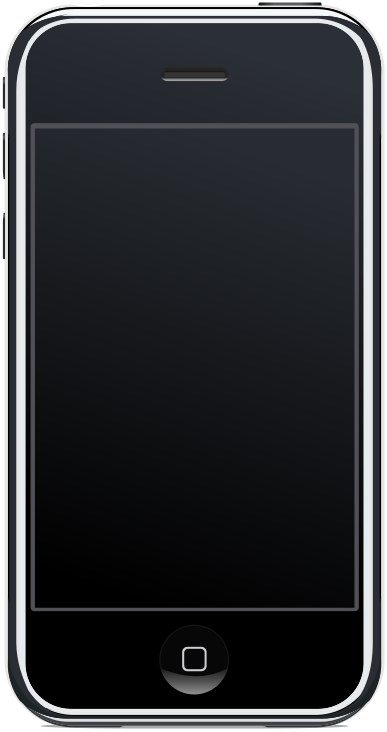
\includegraphics[width=1.5in,height=1in]{iPhone}
			\end{figure}
			\column{4cm}
			\begin{figure}
				\vspace{1em}
				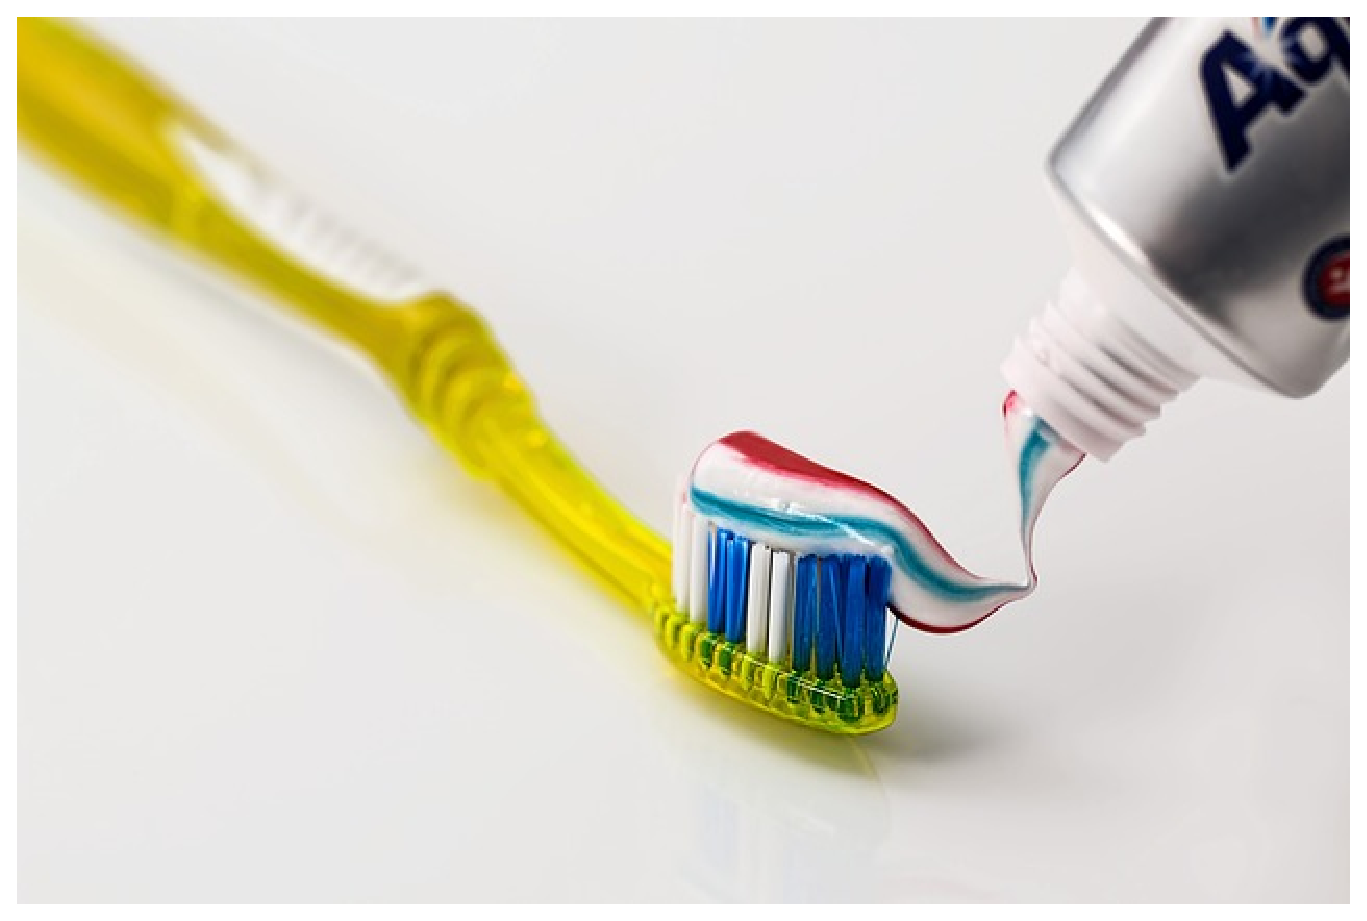
\includegraphics[width=1.5in,height=1in]{toothbrush}
				
			\end{figure}
			
		\end{columns}
		\vspace{1em}
	
	\end{itemize}
	
\end{frame}

\subsection*{Overview}


\begin{frame}
	\frametitle{how to select a reasonable negative item $v_j$ ?}
	\vspace{-2em}
	\begin{columns}
		\column{3cm}
		\begin{figure}
			
\includegraphics[width=1in]{man}
		\end{figure}
		\column{3cm}
		\begin{figure}
			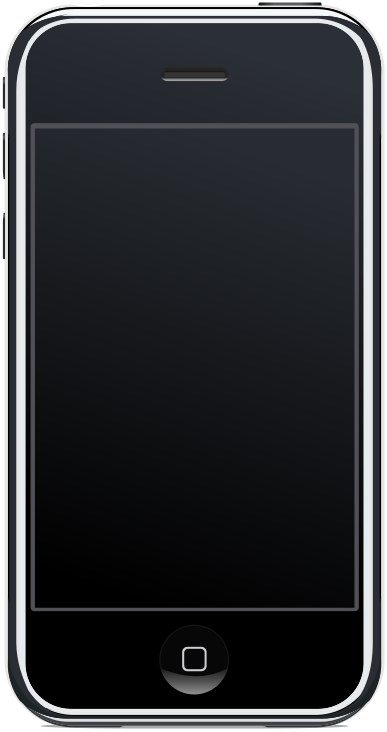
\includegraphics[width=1.5in,height=1in]{iPhone}
		\end{figure}
		\column{4cm}
		\begin{figure}
			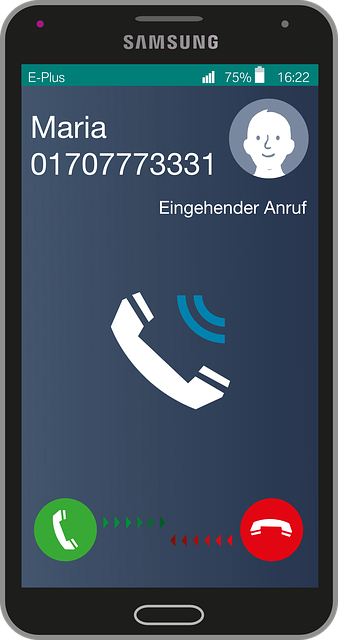
\includegraphics[width=.8in,height=1.5in]{Samsung}
		\end{figure}
	\end{columns}
	\vspace{.5em}
	\begin{columns}
		\pause
		\column{.5\textwidth}
		\begin{block}{First step}
			infer the event that user $u_m$ selected item
			$v_i$ happens on \textcolor{red}{which category}  by the categorical distributions.
		\end{block}
		\column{.5\textwidth}
		\pause
		\begin{block}{Second step}
			select an item $v_j$ with \textcolor{red}{a high probability to be browsed} by user $u_m$ under the selected category.
		\end{block}
	\end{columns}
\end{frame}


\subsection*{Categorical Distribution}
\begin{frame}{Categorical Distribution}
	\begin{itemize}
		\item  The probability that the entity $e_i$ belongs to the category $c \in C$:
		\begin{equation}
		p\left(c|e_i\right)  \propto exp\left( \frac {y_{i,c}^e - \mu_c}{\sigma_c} \right)
		\end{equation}
		where $\mu _c = E\left(y^e_{*,c}\right)$ and $\sigma_c = Var\left(y^e_{*,c}\right)$ denote the empirical mean and variance over all entity factors, respectively.
		
	\end{itemize}
\end{frame}
\begin{frame}{Categorical Distribution}
	\begin{itemize}
		\setlength{\itemsep}{1.5em}
		\item It is assumed that the categorical distributions of users and items
		are independent.
		\item Then, the probability of observed
		user-item pair $(u_m ,v_i )$ associating with the category $c$ could be derived to be a
		joint probability:
		\begin{equation}
		\label{equ:uipair}
		p\left(c|u_m,v_i\right) = p\left(c|u_m\right)p\left(c|v_i\right)
		\end{equation}
	\end{itemize}
\end{frame}





\subsection*{Rank-Invariant of Item List}
\begin{frame}{Rank-Invariant of Item List}
	\begin{itemize}
		
		\item We adopt Geometric distribution to draw the item
		$v_j$ from the ranking list of the category $c$ :
		\begin{equation}
		p\left(v_j|c\right) \propto exp\left(-r\left(j\right)/\lambda\right),\lambda \in \mathbb{R}^+
		\end{equation}
		where $r(j)$ denotes the ranking place of the item $v_j$ , $\lambda$ is
		a hyper-parameter which tunes the probability density.
	\end{itemize}
	
\end{frame}





\subsection*{Discussion of Sorting Items}
\subsection*{Sampling Algorithm}
\begin{frame}

	\begin{figure}
		\includegraphics[width=2in]{subspace}
	\end{figure}
	\begin{itemize}
		\item Based on the study of subspace learning, we can initialize the ranking lists according to content information of items.
	\end{itemize}
	 
\end{frame}
\begin{frame}{Select a popular category}
	\begin{itemize}
		\setlength{\itemsep}{1.5em}
		\item According to Eq(\ref{equ:uipair}), user-item pairs could be arranged into categories.
		\item We further count the
		number of \textbf{observed user-item pairs} under each category, and update the category popularity indicator $\rho$.
		
		
	\end{itemize}
	
\end{frame}

\begin{frame}{Update the popular category}
	\begin{itemize}
		\setlength{\itemsep}{1em}
		\item In each iteration, we first sample a popular category $c$ according
		to its popularity:
		\begin{equation}
		p\left(c|\rho \right) \propto exp\left(\frac{\rho_c - \mu }{\sigma}\right)
		\end{equation}
		where $\mu$ and $\sigma$ denote the empirical mean and variance over
		the variable $\rho$, respectively.
		\item If the change of ranking score vector under category $c$ is over given threshold $\delta$, we update   $x_c$ by $y^v_{*,c}$.
	\end{itemize}
\end{frame}




\begin{frame}
	\begin{figure}
	%	\begin{center}
			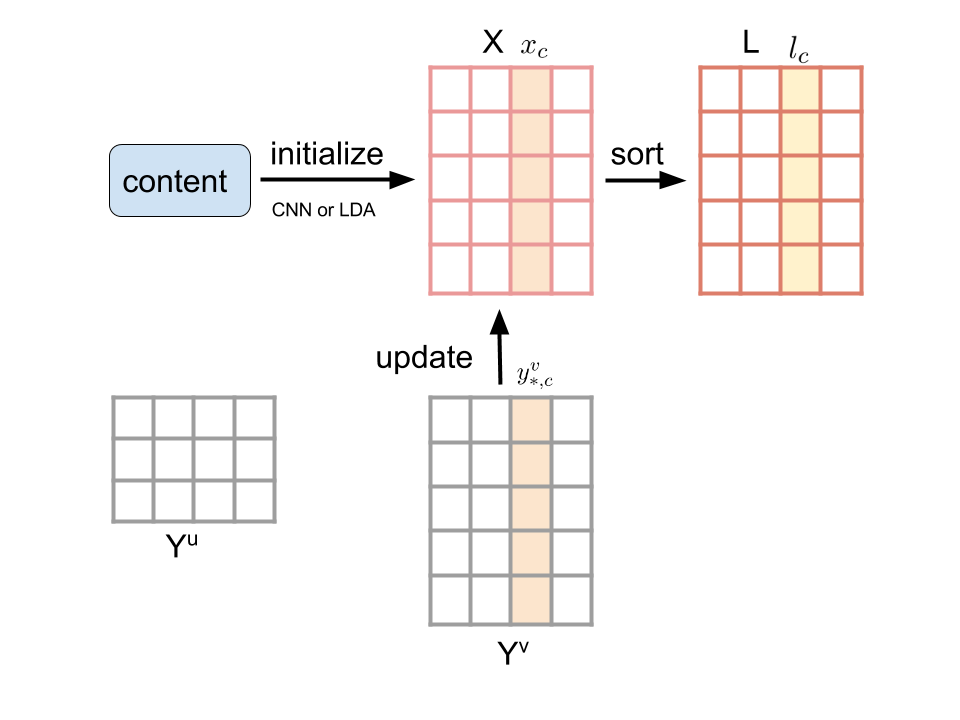
\includegraphics[width=3.5in]{algo2}
	%	\end{center}
	\caption{Adaptive sampling algorithm}
	\end{figure}
\end{frame}


\begin{frame}{Adaptive sampling algorithm}
	\IncMargin{1em}
	\begin{algorithm}[H]%Beamer中的算法排版需要加选项[H]以解决浮动环境问题​
		\SetAlgoNoLine %不要算法中的竖线
		Draw a popular category $c$ from $p\left(c|\rho\right)$\;
		\If {$sim \left(x_c,y_{*,c}^v\right) > \delta $}{
			Update $x_c$ by $y_{*,c}^v$\;
			Reorder items under $c$ and update $l_c$\;
		}
		Draw $\left(u_m,v_i\right) \in \mathcal{P}$ uniformly\;
		Draw a category $c$ from $p\left(c|u_m,v_i\right)$,$\left(1\leq c \leq k\right)$\;
		$\rho_c ++$\;
		Draw a rank $r$ from $p\left(r\right) \propto exp\left(-r/\lambda\right),\left(1\leq c \leq k\right)$\;
		$v_j \leftarrow 
		\begin{cases}
		index\left(c,r\right) & if \ sgn\left(y_{m,c}^u\right) = 1\\
		index\left(c,n-r-1\right) & else
		\end{cases}$\;
		\caption{Content-aware and Adaptive sampling}
		\label{algo:sampling}
	\end{algorithm}
	\DecMargin{1em}
\end{frame}




	\section{预备知识}

\subsection{Bayesian Personalized Ranking}
\begin{figure}[htbp]
	% caption放上面就会显示在图的上方,出现在下面就是出现在图的下方
	% label的位置也有讲究
	\begin{center}
		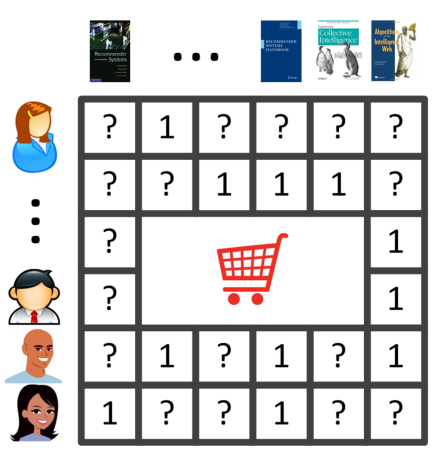
\includegraphics[width=3in]{matrix}
		\caption{user-item 隐式反馈矩阵}
		\label{gra3}
	\end{center}
\end{figure}
在这一节, 我们首先回顾BPR算法,然后讨论它的一些局限性,也就是其收敛缓慢与冷启动问题。通常用户与物品的隐式反馈可以表示为如图\ref{gra3}所示的矩阵, 矩阵的“1”表示用户已经对该物品有过交互行为, 比如购买,点击等, 矩阵的“?”则表示用户还未对该物品有过交互行为。

\subsubsection{Pairwise Preference Assumption}
BPR\cite{rendle2009bpr}是一个应对隐式反馈很流行的推荐框架. 它基于这样一个偏好假设: 如果一个用户$u$已经选择了物品$i$但是没有选择物品$j$,那么在BPR中, 我们认为相对于物品$j$用户$m$更喜欢物品$i$,并定义用户$u$关于物品$i$与$j$的偏好关系为:
\begin{equation}
\label{pairwisepre}
p \left( i \succ_u j \right) := f \left( x_{uij} \right),
\end{equation}
这里$f \left(x\right) = 1/\left(1+exp\left(-x\right)\right)$\footnote{$f \left(x\right)$即为sigmoid函数}, $x_{uij} := s\left(u,i\right) - s\left(u,j\right)$, $s\left(\cdot,\cdot\right)$可以是任何表示用户与物品相关程度的函数。在BPR\cite{rendle2009bpr}中, $s\left(\cdot,\cdot\right)$为用户对物品的预测值, 即$s\left(u,i\right) = \hat{r}_{ui}$, $x_{uij} = \hat{r}_{ui}-\hat{r}_{uj}$.


\subsubsection{预测公式}

在BPR中, 用户$u$对于物品$i$的预测值$\hat{r}_{ui}$公式为:
\begin{equation}
\hat{r}_{ui} = U_{u\cdot}V_{i\cdot}^T + b_i
\end{equation}


\subsubsection{Likelihood of Pairwise Preference}

伯努利分布(Bernouli distribution)是关于布尔变量 $x \in \{0,1\}$ 的概率分布, 其连续参数 $p \in \left[0,1\right]$的概率.
\begin{equation}
\left( x|p \right) = Ber\left(x|p \right)=p^x\left(1-p \right)^{1-x}
\end{equation}

若记事件 $\left(\hat{r}_{ui} > \hat{r}_{uj}\right)$ 的概率为$p\left(\hat{r}_{ui} > \hat{r}_{uj}\right)$, 布尔变量$\delta\left(\left(u,i\right) \succ \left(u,j\right)\right)$ 服从伯努利分布, 那么用户$u$的likelihood of pairwise preference 在\cite{rendle2009bpr}中被定义为:
\begin{equation}
\label{LPP}
\begin{aligned}
LPP_u  
&= \prod_{i,j \ \in \  \mathcal{I}}p\left(\hat{r}_{ui} > \hat{r}_{uj}\right)^{\delta\left(\left(u,i\right) \succ \left(u,j\right)\right)} \left[1-p\left(\hat{r}_{ui} > \hat{r}_{uj}\right)\right]^{1-\delta\left(\left(u,i\right) \succ \left(u,j\right)\right)}\\
&= \prod_{\left(u,i\right) \succ \left(u,j\right)}p\left(\hat{r}_{ui} > \hat{r}_{uj}\right)\prod_{\left(u,i\right) \preceq \left(u,j\right)}\left[1-p\left(\hat{r}_{ui} > \hat{r}_{uj}\right)\right]
\end{aligned}
\end{equation}

这里的$\left(u,i\right) \succ \left(u,j\right)$ 表示用户 $u$ 相比物品 $i$ 更喜欢物品 $j$.

用 $f \left(\hat{r}_{uij} \right)$ 来近似表示概率
$p\left(\hat{r}_{ui} > \hat{r}_{uj}\right)$ \cite{rendle2009bpr}, 对于公式\ref{LPP}取其对数即$\ln LPP_u$, 那么就有:
\begin{equation}
\label{eq5}
\begin{aligned}
\ln LPP_u
&= \ln \prod_{\left(u,i\right) \succ \left(u,j\right)} f \left(\hat{r}_{uij}\right) + \ln \prod_{\left(u,i\right) \preceq \left(u,j\right)}\left[1- f \left(\hat{r}_{uij}\right)\right]\\
&= \ln \prod_{\left(u,i\right) \succ \left(u,j\right)} f \left(\hat{r}_{uij}\right) + \ln \prod_{\left(u,i\right) \succ \left(u,j\right)}\left[1-\left(1- f \left(\hat{r}_{uij}\right)\right)\right]\\
&= \ln \prod_{\left(u,i\right) \succ \left(u,j\right)} f \left(\hat{r}_{uij}\right) + \ln \prod_{\left(u,i\right) \succ \left(u,j\right)} f \left(\hat{r}_{uij}\right)\\
&= 2\ln \prod_{\left(u,i\right) \succ \left(u,j\right)} f \left(\hat{r}_{uij}\right)\\
&= 2 \sum_{i\in\mathcal{I}_u^{tr}}
\sum_{j \in \mathcal{I}\setminus \mathcal{I}_u^{tr}}\ln f \left(\hat{r}_{uij}\right)
\end{aligned}
\end{equation}
在这里$\hat{r}_{uij} = \hat{r}_{ui} - \hat{r}_{uj}$, $f \left(x\right) = 1/\left(1+exp\left(-x\right)\right)$, .

\subsubsection{目标函数}

基于上面的成对偏好假设,可以从隐式反馈数据集中得到所有的偏好集合$D_S := \{\left(u,i,j\right) | v_i \in I_{u}^+ \wedge v_j \in I \setminus I_{u}^+\}$,$I_m^+$表示被用户$u$选择过的物品集合,三元组$\left(u,i,j\right)$表示用户$u$选择过物品$v_i$但是没有选择过物品$v_j$。我们把$v_i$叫做一个positive item,$v_j$叫做一个negative item。对于给定的集合$D_S$, BPR的目标便是最大化所有user-item pair的似然偏好:

\begin{equation}
\label{eq6}
arg \max_{\substack \Theta } \prod_{\left(u,i,j\right) \in D_S} p\left(i \succ_u j\right),
\end{equation}

公式\eqref{eq6}等价于最小化负的对数似然函数:

\begin{equation}
\label{Lfeedback}
L_{feedback} = - \sum_{\left(u,i,j\right) \in D_S}\ln f \left( x_{uij}\right) + \lambda\|\Theta\|^2,
\end{equation}
这里的$x_{uij} = \hat{r}_{uij}$, $\Theta$表示算法中需要学习的模型参数集合,$\lambda$表示超参数集合。在实际的算法学习中, BPR的学习算法经常采用均匀采样的随机梯度下降(\textbf{S}tochastic \textbf{G}radient \textbf{D}escent)进行迭代学习。

更为具体的,公式\eqref{Lfeedback}也就是最小化下面的目标函数(Objective Function): 
\begin{equation}
\label{eq8}
\min_{\substack\Theta}\sum_{u\in\mathcal{U}} \ \sum_{i\in\mathcal{I}_u}\sum_{j\in\mathcal{I}\setminus\mathcal{I}_u}\Phi_{uij}
\end{equation}
这里的
$\Phi_{uij}
= 
- \ln f \left(\hat{r}_{uij}\right) 
+ \frac{\alpha_u}{2}\|U_{u\cdot}\|^2
+ \frac{\alpha_v}{2}\|V_{i\cdot}\|^2
+ \frac{\alpha_v}{2}\|V_{j\cdot}\|^2
+ \frac{\beta_v}{2}\|b_{i}\|^2
+ \frac{\beta_v}{2}\|b_{j}\|^2$, $\Theta = \{U_{u\cdot},V_{i\cdot},b_i\}
$的将要学习的参数集合。


\subsubsection{随机梯度}
对于一个随机采样而得的三元组$\left(u,i,j\right)$, 对目标函数中的参数求其偏导即可得梯度。

在此之前先做一些准备工作,对于函数$f(x) = 1/\left(1+e^{-x}\right)$的导数:

\begin{equation*}
f^{'}(x) = -\frac{1}{\left(1+e^{-x}\right)^2} e^{-x}\left(-1\right) = \frac{e^{-x}}{\left(1+e^{-x}\right)^2} = \frac{1}{\left(1+e^{x}\right)\left(1+e^{-x}\right)} = {f(x)f(-x)}
\end{equation*}

下面开始对参数$U_{u\cdot}$求其偏导:
\begin{equation}
\begin{aligned}
\bigtriangledown U_{u\cdot} 
= \frac{\partial \Phi_{uij}}{\partial U_{u\cdot}}
&=-\frac{\partial \ln f\left(\hat{r}_{uij}\right)}{\partial f\left(\hat{r}_{uij}\right)} 
\frac{\partial f\left(\hat{r}_{uij}\right) }{\partial \hat{r}_{uij}} 
\frac{\partial \hat{r}_{uij}}{\partial U_{u\cdot}}
\ + \  \alpha_uU_{u\cdot}\\
&= -\frac{1}{f\left(\hat{r}_{uij}\right)} 
\frac{\partial f\left(\hat{r}_{uij}\right) }{\partial \hat{r}_{uij}} 
\frac{\partial \hat{r}_{uij}}{\partial U_{u\cdot}}
\ + \  \alpha_uU_{u\cdot}\\
&= -\frac{1}{f\left(\hat{r}_{uij}\right)} 
{f\left(\hat{r}_{uij}\right) f\left(-\hat{r}_{uij}\right)}
\frac{\partial f\left(\hat{r}_{ui} - \hat{r}_{uj}\right) }{\partial U_{u\cdot}} 
\ + \ \alpha_uU_{u\cdot}\\
&= -{f\left(-\hat{r}_{uij}\right)} \frac{\partial f\left[\left(U_{u\cdot}V_{i\cdot}^T+b_i\right) - \left(U_{u\cdot}V_{j\cdot}^T+b_j\right)\right] }{\partial U_{u\cdot}} 
\ + \ \alpha_uU_{u\cdot}\\
&= -{f\left(-\hat{r}_{uij}\right)} \left(V_{i\cdot} - V_{j\cdot}\right)  
\ + \  \alpha_uU_{u\cdot}\\
\end{aligned}
\end{equation}

同样其他参数随机梯度如下:
%\begin{equation}
\begin{align} %align环境不要有空行
\bigtriangledown V_{i\cdot} &= \frac{\partial \Phi_{uij}}{\partial V_{i\cdot}}=-f\left(-\hat{r}_{uij}\right)U_{u\cdot} + \alpha_vV_{i\cdot}\\
\bigtriangledown V_{j\cdot} &= \frac{\partial \Phi_{uij}}{\partial V_{j\cdot}}=-f\left(-\hat{r}_{uij}\right)\left(-U_{u\cdot}\right) + \alpha_vV_{j\cdot}\\
\bigtriangledown b_i        &= \frac{\partial \Phi_{uij}}{\partial b_i} =-f\left(-\hat{r}_{uij}\right)+\beta_vb_i\\
\bigtriangledown b_j        &= \frac{\partial \Phi_{uij}}{\partial b_j} =-f\left(-\hat{r}_{uij}\right)\left(-1\right)+\beta_vb_j
\end{align}
%\end{equation}

\subsubsection{迭代更新}
对于三元组  $\left(u,i,j\right)$ 在采用SGD的BPR算法中的更新公式如下:
%align环境的每行公式默认会进行编号,aligned环境不会
\begin{align}
	\label{eq10}
U_{u\cdot} &= U_{u\cdot} - \gamma\bigtriangledown U_{u\cdot}\\
V_{i\cdot} &= V_{i\cdot} - \gamma\bigtriangledown V_{i\cdot}\\
V_{j\cdot} &= V_{i\cdot} - \gamma\bigtriangledown V_{j\cdot}\\
b_{i\cdot} &= b_i - \gamma\bigtriangledown b_{i}\\
b_{j\cdot} &= b_j - \gamma\bigtriangledown b_{j}
\end{align}

这里的 $\gamma$ 为学习率(learning rate).

\subsubsection{BPR算法}
如算法\ref{al1}即为采用SGD求解的BPR算法。
\IncMargin{1em}
\begin{algorithm}[ht]
	\SetAlgoNoLine %不要算法中的竖线
	\BlankLine
	
	initialize the model parameter $\Theta$\;
	\For {$t_1 = 1,\cdots,T$}{
		\For {$t_2 = 1,\cdots, |\mathcal{P}|$}{
			Randomly pick up a pair $\left(u,v_i\right) \in \mathcal{P}$\;
			Randomly pick up an item $v_j$ from $\mathcal{I} \setminus \mathcal{I}_{u}^+$\;
			Calculate the gradients via Eq.(9-13)\;
			Update the model parameters via Eq.(14-18)\;
		}	
	}
	\caption{The SGD algorithm for BPR}
	\label{al1}%label 放置的位置有讲究, 放后面
\end{algorithm}
\DecMargin{1em}

\subsubsection{收敛缓慢的原因}
由于上面的均匀采样方式会产生很多对于参数学习贡献微弱的train pairs,因此常常会导致收敛缓慢。确切的讲,对于一个给定的训练采样$\left(u,i,j\right) \in D_S$, 由公式\ref{Lfeedback}对随机梯度下降的任意一参数$\theta \in \Theta$求其偏导:

\begin{equation}
\label{eq19}
\frac {\partial L_{feedback}} {\partial\theta} 
= -f\left(-x_{uij}\right)\frac{\partial\left(x_{uij}\right)}{\partial\theta}
= \left(f\left(x_{uij}\right)-1\right) \frac{\partial\left(x_{uij}\right)}{\partial\theta}
\end{equation}

根据公式\eqref{eq19},如果$f \left(x_{uij}\right) \rightarrow +1$,随机梯度将接近于0,则训练采样$\left(u,i,j\right)$对于优化目标的贡献将会变得很小。
\begin{figure}[htbp]
	\begin{center}
		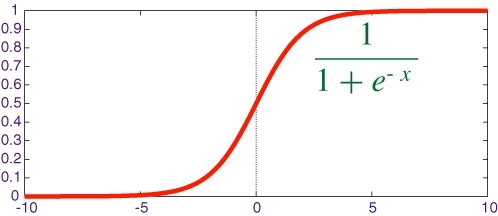
\includegraphics[width=4in]{sigmoid}
		\caption{sigmoid函数$f \left(x\right) $图像}
		\label{gra-sigmoid}
	\end{center}
\end{figure}

联系公式\eqref{eq19}与公式\eqref{pairwisepre},由图\ref{gra-sigmoid} sigmoid函数图像可得, 当$f \left(x_{uij}\right) \rightarrow +1$时, 也就是$x_{uij} = \hat{r}_{ui} - \hat{r}_{uj}$越来越大, 即用户对于物品$v_i$与$v_j$的预测差值越来越大. 因此为了加速学习, 针对一个已有的user-item pair中的物品 $v_i$,要采样的物品$v_j$应当是$v_i$相比有竞争力的物品, 更进一步说也就是由该用户对于$v_i$与$v_j$的偏好得分应该是相近的,否则这个采样对于SGD便是低效的采样。

从经验上来讲,每个用户只会浏览一小部分的物品并对这些浏览过的物品提供一些交互反馈。如果均匀采样器均等地从整个物品集合中采样negative  item.对于一个user-item  pair,大部分均匀采样的物品并不具有可比性或者很难被相关的用户浏览。举个例子,iPhone与牙刷或iPhone与一个冷门的手机品牌可能会经常被均匀采样器采得。而由于这些低效的training pair对于SGD几乎作用很小,整个训练过程便会收敛地极其缓慢。

除此以外,与经典的分解技术相似,如果一个用户或物品缺乏足够的反馈,其对应的隐式表达往往不能够被很好的学习到。在现实世界数据集中,用户行为与物品流行度的分布往往呈现长尾状。这就导致了大部分的用户和物品仅仅有很小部分的反馈数据。此外,在真实的推荐系统中,新的个体可能在任何时间被加入到推荐系统中。因此,BPR框架也很容易受制于冷启动问题。

\subsection{Latent Dirichlet Allocation}
Latent Dirichlet allocation(LDA),隐含狄利克雷分布,是一种主题模型(topic model),它可以将文档集中每篇文档的主题按照概率分布的形式给出。同时它是一种无监督学习算法,在训练时不需要手工标注的训练集,需要的仅仅是文档集以及指定主题的数量即可。此外LDA的另一个优点则是,对于每一个主题均可找出一些词语来描述它。

LDA首先由于2003年提出\cite{blei2003latent},目前在文本挖掘领域包括文本主题识别、文本分类以及文本相似度计算方面都有应用。


\subsubsection{数学模型}
LDA是一种典型的词袋(Bag-of-words)模型,即它认为一篇文档(document)是由一组词(word)构成的一个集合,词与词之间没有顺序以及先后的关系。一篇文档可以包含多个主题(topic),文档中每一个词都由其中的一个主题生成。

\begin{figure}[htbp]
	% caption放上面就会显示在图的上方,出现在下面就是出现在图的下方
	% label的位置也有讲究
	\begin{center}
		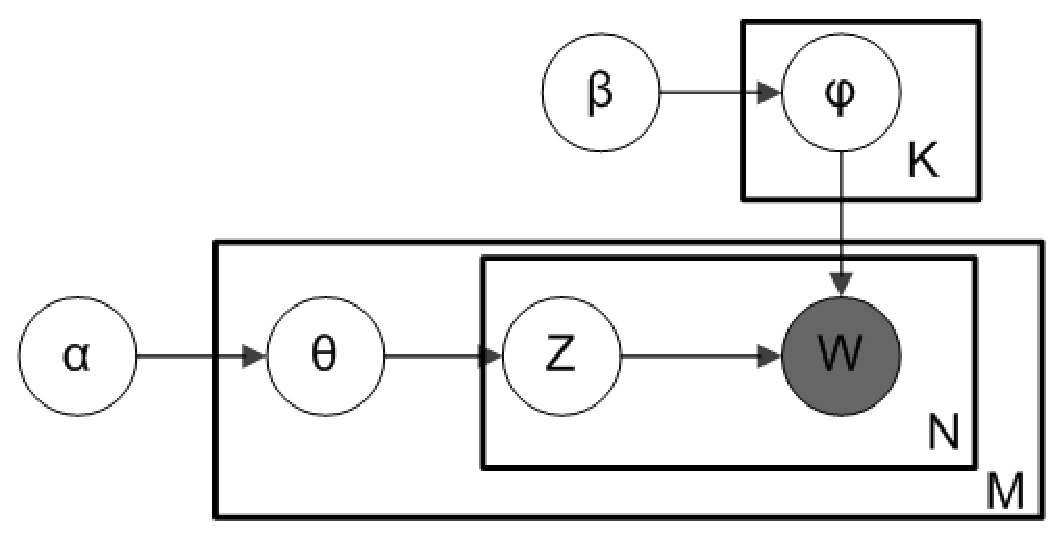
\includegraphics[width=4in]{LDA}
		\caption{LDA 贝叶斯网络结构}
		\label{gra4}
	\end{center}
\end{figure}

另外,正如Beta分布是二项式分布的共轭先验概率分布,狄利克雷分布作为多项式分布的共轭先验概率分布。因此正如图\ref{gra4}, LDA贝叶斯网络结构中所描述的,在LDA模型中一篇文档生成的方式如下:
\begin{itemize}
	\item 从狄利克雷分布$\alpha$ 中取样生成文档$i$的主题分布$\theta_i$
	\item 从主题的多项式分布$\theta_i$中取样生成文档$i$第$j$个词的主题$z_{i, j}$
	\item 从狄利克雷分布$\beta $中取样生成主题$z_{i, j}$的词语分布$\phi_{z_{i, j}}$
	\item 从词语的多项式分布$\phi_{z_{i, j}}$中采样最终生成词语$w_{i, j}$
\end{itemize}
因此整个模型中所有可见变量以及隐藏变量的联合分布是
\begin{equation}
p(w_i, z_i, \theta_i, \Phi | \alpha, \beta) = \prod_{j = 1}^{N} p(\theta_i|\alpha)p(z_{i, j}|\theta_i)p(\Phi|\beta)p(w_{i, j}|\theta_{z_{i, j}})
\end{equation}


最终一篇文档的单词分布的最大似然估计可以通过将上式的$\theta_i$以及$\Phi$进行积分和对$z_i$进行求和得到
\begin{equation}
p(w_i | \alpha, \beta)  = \int_{\theta_i}\int_{\Phi }\sum_{z_i}p(w_i, z_i, \theta_i, \Phi | \alpha, \beta) 
\end{equation}


根据$p(w_i | \alpha, \beta)$ 的最大似然估计,最终可以通过吉布斯采样等方法估计出模型中的参数。


\subsubsection{使用吉布斯采样估计LDA参数}
在LDA最初提出的时候,人们使用EM算法(Expectation-maximization algorithm)进行求解,后来人们普遍开始使用较为简单的Gibbs Sampling,具体过程如下:
\begin{itemize}
	\item 首先对所有文档中的所有词遍历一遍,为其都随机分配一个主题,即$z_{m,n}=k\sim Mult(1/K)$,其中$m$表示第$m$篇文档,$n$表示文档中的第$n$个词,$k$表示主题,$K$表示主题的总数,之后将对应的$n^{\left(k\right)}_m+1$, $n_m+1$, $n^{\left(t\right)}_k+1$, $n_k+1$, 他们分别表示在$m$文档中$k$主题出现的次数,$m$文档中主题数量的和,$k$主题对应的$t$词的次数,$k$主题对应的总词数。
	\item 之后对下述操作进行重复迭代。
	\item 对所有文档中的所有词进行遍历,假如当前文档$m$的词$t$对应主题为$k$,则$n^{\left(k\right)}_m-1$, $n_m-1$, $n^{\left(t\right)}_k-1$, $n_k-1$, 即先拿出当前词,之后根据LDA中topic sample的概率分布sample出新的主题,在对应的$n^{\left(k\right)}_m$, $n_m$, $n^{\left(t\right)}_k$, $n_k$上分别$+1$。
	\begin{equation}
	p(z_i=k|z_{-i},w) \propto k(n^{(t)}_{k,-i}+\beta_t)(n_{m,-i}^{(k)}+\alpha_k)/(\sum_{t=1}^{V}n_{k,-i}^{(t)}+\beta_t)
	\end{equation}
	\item 迭代完成后输出主题--词参数矩阵$\Phi$和文档--主题矩阵$\Theta$
	\begin{align}
	\phi_{k,t}   &=(n_k^{(t)}+\beta_t)/(n_k+\beta_t)  \\
	\theta_{m,k} &=(n_m^{(k)}+\alpha_k)/(n_m+\alpha_k)
	\end{align}
\end{itemize}









\subsection{本章小结}
本章首先介绍了采用SGD求解的Bayesian Personalized Ranking(BPR)推荐算法, 并且对可能导致其收敛缓慢的均匀采样策略做了讨论。然后简要介绍了LDA模型。
	\section{适应性采样策略}
在这一章中,我们结合了内容信息与隐式反馈提出了一个非均匀的物品采样器(a non-uniform item sampler)。在本章中所提出的适应性采样策略(adaptive sampling strategy)自动地模拟了真实的数据分布并且具有适应性地挑选更有针对性的train pairs.


\subsection{适应性采样策略概览}
在现实世界的场景中,用户常常会浏览同一个目录下的多个物品,然后做出他们的选择。那么很显然,我们应该采样具有针对性的物品,比方说针对iPhone,相对于毛巾或者某低档品牌的手机, 采样高档Samsung或者LG显然更具有可比性与合理性。

因此,在适应性采样策略中,我们倾向于采样那些对于用户已选择过的物品更具有可比性同时有很大机会被相关用户浏览的物品。更确切的说,对于一个user-item pair$\left(u_m,v_i\right)$,我们通过以下的步骤采样一个更加合理的负样本(negative item)$v_j$:
\begin{enumerate}
	\item 根据用户$u_m$与物品$v_i$的所在目录分布(categorical distribution),首先推断对于事件用户$u_m$选择物品$v_i$会发生在哪个目录下。
	\item 
	对于给定的一个目录,在该目录下我们进一步选择物品$v_j$作为negative item,而该物品同时又具有较高的概率能够被用户$u_m$所浏览。
\end{enumerate}




\subsection{类别分布}
在适应性采样中, 首先需要知道用户与物品的类别分布(categorical distribution). 不过在有些实际的应用场景中,由于缺乏类别信息,推荐系统并无法直接得到用户与物品的类别分布。为了应对这个问题,我们利用了所谓的隐式表达(the latent representation of an entity)来近似指示其类别信息。

首先我们假设一个entity可能属于多个目录 $C = \{c_1,c_2,\cdots,c_k\}$ ,并且它的类别分布服从幂率(power laws)分布\cite{rendle2014improving}. 用$y_i^e \in \mathbb{R}^k$ 表示 entity $e_i$ 的latent vector ,而矩阵 $Y_e = \left[y_1^e,y_2^e,y_3^e,\cdots\right]$ 是从内容信息(content information)与隐式反馈(implicit feedback)学习得到的entities's latent representation. 以推荐系统中的一个经典场景为例:在推荐系统有两种类型的实体(entity),也就是说用户users, 比如消费者, 和物品items, 比如说电影,书籍和歌曲等。明确起见,本论文使用上标$u$与$v$分别表示与用户user和物品item相关的变量。比如,$y^u_m$表示the latent vector of user $u_m$,$Y^u$表示the latent representation matrix of user, $y_i^v$表示the latent vector of item $v_i$.为了联系categorical distribution 与 the latent vector of entity, 我们认为 entity $e_i$属于目录$c\in C$的概率$p\left(c|e_i\right)$为标准化因子的混合(a mixture over standardized factors),并将其定义为:

\begin{equation}
p\left(c|e_i\right)  \propto exp\left( \frac {y_{i,c}^e - \mu_c}{\sigma_c} \right)
\end{equation}

这里的$\mu_c = E\left(y_{*,c}^e\right)$,$\sigma_c = Var\left(y_{*,c}^e\right)$分别表示all entity factors的经验均值与方差(empirical mean and variance over all entity factors)。假设在用户与物品上的类别分布是相互独立的,那么就可以进一步推断user-item pair$\left(u_m,v_i\right)$同属于一个category $c$的联合概率$p\left(c|u_m,v_i\right)$:

\begin{equation}
\label{eq21}
p\left(c|u_m,v_i\right) = p\left(c|u_m\right)p\left(c|v_i\right)
\end{equation}

根据其联合概率,就可以根据时间用户$u_m$选择物品$v_i$采样一个目录$c$。




\subsection{选取negative item $v_j$}
对于给定一个目录$c$,下一步的目标便是在该目录下选取一个negative item $v_j$,而$v_j$同时将有很大概率会被用户$u_m$所浏览. 

\subsubsection{物品浏览概率}
一个简单点的做法,我们可以将entity $e_i$在目录$c$下的排序得分(ranking score)视作为$p\left(c|e_i\right)$,再进一步从根据它们的排序得分直接选择物品。但实际上,浏览概率(browsing probabilities)与排序得分(ranking scores)并不等同,显然两者之间存在差距。在实际场景中,对于出现在排序列表(ranking lists)中的物品,那些排在靠前位置的物品相对于靠后位置的物品, 往往有着极大的概率被用户所浏览。比如在整个列表中排名前三位的物品的极有可能都会被用户所浏览,而他们排序得分不同的影响在这种情况下将微乎其微。为了应对这个问题,对于给定目录下的物品采样我们分为两步进行:
\begin{enumerate}
	\item 首先,我们先根据经验分布(empirical distribution)从候选物品(candidates)中采样一个排序的位置$r$;
	\item 然后,在该目录下对物品进行排序,返回在位置$r$处的物品作为我们采样的negative item。
\end{enumerate} 

典型地,经验分布大致服从analytical law, 比如Geometric\cite{wang2009pskip}或Zipf\cite{adamic2002zipf} distribution。在这里,我们应用Geometric distribution到从目录$c$的排序列表中选取位置$r(j)$处的物品$v_j$:

\begin{equation}
p\left(v_j|c\right) \propto exp\left(-r\left(j\right)/\lambda\right),\lambda \in \mathbb{R}^+
\end{equation}

这里的$r\left(j\right)$表示物品$v_j$的排序位置,$\lambda$是用来调整概率密度的超参数(hyper-parameter)。




\subsubsection{如何对物品列表进行排序}
在获得negative item的排序位置后,接下来的任务便是如何在这个位置安排对应的物品。\cite{rendle2014improving}中有一个简单的方法:将物品的 latent factors 当作其 ranking scores, 然后根据它们的排序得分(ranking scores)对物品进行排序. 但是由于物品的latent factors在每轮迭代都会被更新,这种方法不得不在每轮迭代每个目录下对物品进行重新排序。这会导致一个很高的计算复杂度,因为每轮迭代需要花费$\mathit{O}\left(kt\log t\right)$的运行时间来进行重新排序,这里的$t$指物品数。为此在\cite{rendle2014improving}中同样提出一个妥协性的做法:每迭代$t \log t$轮再进行重新排序。不过这种妥协会很容易导致局部收敛(local convergence)。此外, 每隔$t\log t$轮进行更新, 实际上在很多未更新的时候的采样相当于从一个随机的物品子集中随机采样, 此时的采样反而会产生副作用。更进一步, 由于items' latent vectors 是被随机初始化, 那么排序列表在首次重排序之前其实是相当于一个随机序列。如果这个随机的排序列表未被及时更新, 那么采样器实际上会衰退为从一个物品子集中随机采样的采样器。因此, 需要一个新的采样方法来平衡效率与推荐表现。

\begin{figure}[htbp]
	\begin{center}
		\includegraphics[width=3.5in]{subspace}
		\caption{将不同模态(different modalities)的entity映射到一个共享的隐式空间(a shared latent space). 在这里假设协同信息(collaborative information), 比如评分(rating), 和内容信息(content information), 比如文本(text),分属于不同模态,正如图中的space A, space B.}
		\label{gra5}
	\end{center}
\end{figure}

根据对于子空间的研究\cite{udupa2010improving,rasiwasia2010new},如果我们将一个entity从不同模态的映射到一个共享子空间,那么它在子空间中的表达应当是具有关联性的,比如互补(complementary)或是相似(similar)。如果我们独立地将一个item从content space和collaborative space映射到a shared latent space,那么我们就能够得到一个item在共享隐式空间的两个latent representations.如图\ref{gra3}所示. 为了避免采样器衰退为从一个物品子集中随机采样一个物品, 我们通过物品的协同信息(collaborative filtering)来初始化排序列表(ranking lists)。具体来说, 我们首先通过特征学习(feature learning)的方法从协同信息中学习物品的一个近似的隐式表达(latent representation), 比如, 用于图像的Conventional Neural Networks(CNN), 用于文本的Latent Dirichlet Allocation(LDA)。那么, 我们将latent factors视作为在目录分布下的物品排序得分, 然后在每个目录下对物品进行排序. 最终, 我们就根据这些排序后的结果对物品排序列表进行初始化。

此外, 为了避免局部收敛的问题, 同时平衡效率, 我们\textbf{只对于那些热门目录下的物品进行重排序}。根据公式\eqref{eq21}, 首先对于一个user-item pair选定一个目录, 然后进一步计算在每个目录下出现了多少所观测的user-item pairs.定义变量$\rho \in \mathbb{R}^k$来表示目录的热度(popularity of categories)。在每次迭代中, 我们根据目录的热度采样出一个热门目录(popular category) $c$:
\begin{equation}
p\left(c|p\right) \propto exp\left(\frac{\rho_c - \mu }{\sigma}\right)
\end{equation}
这里的$\mu$ 和$\sigma$分别表示$\rho$的经验均值与方差(empirical mean and variance). 然后, 我们将物品的current latent factors视为物品的new ranking scores, 并衡量在目录$c$下的new score vector, 根据a similarity function $sim\left(\cdot,\cdot\right)$与旧的score vector相比是否有较大变化.如果ranking score vector的变化超过了阈值 $\delta$, 就用物品的latent represenration matrix 的第$c$列$y_{*,c}^v$来更新在目录$c$下的ranking scores, 并且对该目录下的物品进行重新排序.

\subsection{适应性采样算法}


总言之,在本论文中所研究的适应性采样策略如算法$\ref{al2}$所示, 对于一个user-item pair$\left(u_m,v_i\right)$, 采样一个negative item $v_j$, 而$v_j$与$v_i$相比, 不仅具有可比性,而且具有较高的几率为用户所浏览。在算法$\ref{al2}$中, $index\left(c,r\right)$返回在排序列表$l_c \in L$中位置在$r$处的物品。$x_c \in X$是在目录$c$下的ranking score vector, 而$x_c$正是由从协同信息学习而来approximate latent representation所初始化。值得注意的是, 在整个学习过程中,本论文的适应性采样策略仅需要在一些热门目录重排序几次, 这不仅降低了计算复杂度同时避免了局部极值(local extremum)。

\IncMargin{1em}
\begin{algorithm}
	\SetAlgoNoLine %不要算法中的竖线
	
	\SetKwInOut{Input}{\textbf{输入}}\SetKwInOut{Output}{\textbf{输出}}
	
	\Input{
		\\
		The observed user-item pair set $\mathcal{P}$\;\\
		The counters of category popularity $\rho$\;\\
		The latent representation matrixes $Y^u$ and $Y^v$\;\\
		The ranking scores of items $X = \{x_1,x_2,\cdots,x_k\}$\;\\
		The orders of items $L = \{l_1,l_2,\cdot,l_k\}$\;\\}
	\Output{
		\\
		The training triple $\left(u_m,v_i,v_j\right)$\;\\
		The category popularity $\rho$\;\\
		Draw a category from $p\left(c|\rho\right)$\;\\}
	\BlankLine
	 Draw a popular category $c$ from $p\left(c|\rho\right)$\;
	 \If {$sim \left(x_c,y_{*,c}^v\right) > \delta $}{
		 Update $x_c$ by $y_{*,c}^v$\;
		 Reorder items under $c$ and update $l_c$\;
	 }
	 Draw $\left(u_m,v_i\right) \in \mathcal{P}$ uniformly\;
	 Draw a category $c$ from $p\left(c|u_m,v_i\right)$,$\left(1\leq c \leq k\right)$\;
	 $\rho_c ++$\;
	 Draw a rank $r$ from $p\left(r\right) \propto exp\left(-r/\lambda\right),\left(1\leq c \leq k\right)$\;
	  
	 $v_j \leftarrow 
	 \begin{cases}
	 index\left(c,r\right) & if \ sgn\left(y_{m,c}^u\right) = 1\\
	 index\left(c,n-r-1\right) & else
	 \end{cases}$\;
	 
	\caption{Content-aware and Adaptive sampling}
	\label{al2}
\end{algorithm}
\DecMargin{1em}




\subsection{本章小结}
本章主要介绍了适应性采样策略, 该采样策略通过采样一个具有可比性同时又有较大概率被用户浏览的物品作为negative item。该采样策略不仅能够降低计算复杂度同时能够避免局部极值。
	
	
	
	\bibliographystyle{apalike}
	\bibliography{ref/presentation}
		
\end{document}